Глава содержит математическую постановку задачи и описание метода решения. Рассматриваются существующие способы постановки краевых условий и предлагается альтернативный способ замыкания системы уравнений. В конце дается краткое описание метода неполной аппроксимации минимальных невязок.
\addtocounter{section}{1}
\setcounter{subsection}{0}
\setcounter{equation}{0}
\section*{Постановка задачи}
\addtocontents{toc}{\contentsline{section}{\protect\numberline{\S\;\thesection.}\vspace{10pt}Постановка задачи}{\thepage}}
Исследуется задача о движении волн на поверхности безграничной идеальной несжимаемой жидкости, которая находится в однородном поле сил тяжести. Течение является потенциальным, т.е. для вектора скорости $\vec{u}=\{u,v,w\}$ существует $\phi(x,y,z,t):\vec{u}=grad \phi$. Введём прямоугольную декартову систему координат так, что ось $Oz$ направлена вертикально вверх, в сторону, противоположную направлению ускорения свободного падения, а оси $Ox$ и $Oy$ лежат на невозмущённой свободной поверхности (рис.\;\ref{figure:schema}). Жидкость заполняет область $Q$, ограниченную сверху свободной поверхностью $z=\eta(x,y,t)$, снизу — дном $z=-\tilde{H}(x,y,t)=-H(x,y)+B(x,y,t)$. Здесь $H$ определяет неподвижную часть дна, а $B$ - его динамическую составляющую.

\begin{figure}[htp]
    \centering
    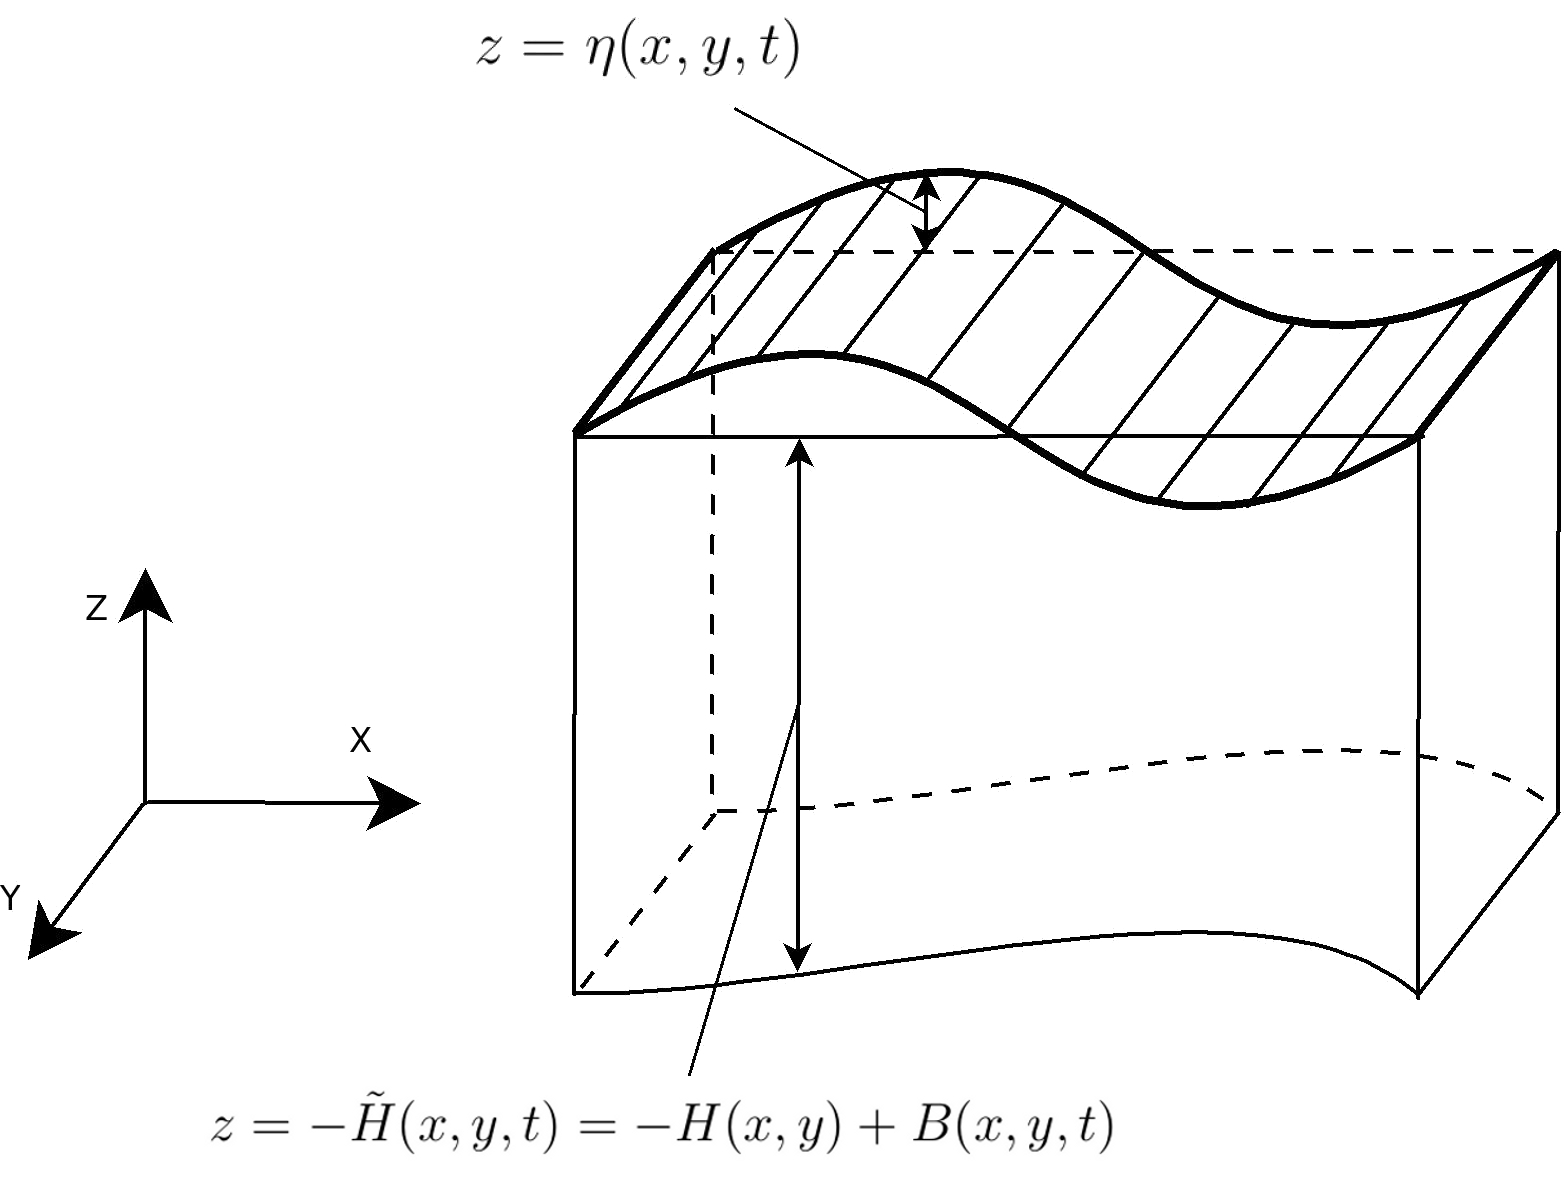
\includegraphics[width=9cm,height=6cm]{scheme.jpg}
    \caption{Постановка задачи}
    \label{figure:schema}
\end{figure}

В качестве физической модели, описывающей данную задачу, взяты уравнения теории мелкой воды (в линейной форме известные также как уравнения Сен-Венана), для которых существенными являются предположения о малости вертикального ускорения частиц жидкости по отношению к ускорению свободного падения и о слабой зависимости горизонтальных скоростей от вертикальной координаты.

Ситуации, когда глубина акватории много меньше горизонтальных размеров, достаточно обычна, поэтому уравнения мелкой воды находят широкое применение. Часто они используются с учётом кориолисовых сил при моделировании атмосферы и океана как упрощение системы примитивных уравнений, описывающих потоки в атмосфере.

Представим уравнения мелкой воды в следующей форме:
\begin{gather}
    \label{eq:MainVectorForm}
    \frac{\partial U}{\partial t}+F_{lin}+F_{nonlin}=\frac{\partial B}{\partial t}\\
    \label{eq:UB}
    U=\begin{pmatrix}\eta\\u\\v\end{pmatrix}
    B=\begin{pmatrix}B(x,y,t)\\0\\0\end{pmatrix}\notag
\end{gather}

\begin{gather}
    \label{eq:FLin}
    F_{lin}=\begin{pmatrix}
	\frac{\partial ((H-B)u)}{\partial x}+\frac{\partial ((H-B)v)}{\partial y}\\
	g\frac{\partial \eta}{\partial x}\\
	g\frac{\partial \eta}{\partial y}
    \end{pmatrix}\\
    \label{eq:FNonLin}
    F_{nonlin}=\begin{pmatrix}
	0\\
	\frac{1}{2}\frac{\partial (u^2)}{\partial x} + v\frac{\partial u}{\partial y}\\
	\frac{1}{2}\frac{\partial (v^2)}{\partial y} + u\frac{\partial v}{\partial x}
    \end{pmatrix}
\end{gather}

%Boundary
\begin{gather}
    \begin{split}
	\label{eq:BoundaryCondition}
	(x,y)&\in\Omega,t>0\\
	u_0=u(x,y,0)\;v_0=&v(x,y,0)\;\eta_0=\eta(x,y,0)\\
	u(x,y,t),v(x,y,t),\eta(&x,y,t)\to0\; x^2+y^2\to\infty
    \end{split}
\end{gather}

	Где $H$ определяет неподвижную часть дна, а $B$ - его динамическую составляющую ($H-B$ – полная грубина слоя жидкости), $\eta$ – функция свободной поверхности, $u(x,y,t)$ – скорость по Ox, $v(x,y,t)$ - скорость по Oy, $g=9,8$. 

	Данные формулы являются гиперболической системой дифференциальных уравнений и описывают более общую постановку задачи в нелинейном виде без учёта сил Кориолиса, трения и вязкости в бесконечной области (более подробно об уравнениях мелкой воды см. \cite{ovsjannikov},\cite{marchyk}). Линейная форма может быть получена как частный случай - для этого достаточно отбросить $F_{nonlin}$.

\newpage
\addtocounter{section}{1}
\setcounter{subsection}{0}
\setcounter{equation}{0}
\section*{Аппроксимация уравнений}
\addtocontents{toc}{\contentsline{section}{\protect\numberline{\S\;\thesection.}\vspace{10pt}Аппроксимация уравнений}{\thepage}}

Задача (\ref{eq:MainVectorForm}), (\ref{eq:BoundaryCondition}) решалась методом сеток. Для решения в расчетной области $\Omega$ введем обычным образом неравномерную в общем случае сетку $\Omega_h$ с шагом $h_{x i}=x_{i+1}-x_{i},h_{y i}=y_{i+1}-y_{i}$ и шагом по времени $\tau=t^{n+1}-t^n$. $n$-й слой по времени определим как множество узлов $(i,j)$ при фиксированном $t^n$.

Обозначим значение сеточной функции $\phi$ в узле $(i,j)$, как $\phi^n_{ij}=\phi(x_i,y_i,t^n)$ и аппроксимируем уравнения (\ref{eq:MainVectorForm}), (\ref{eq:BoundaryCondition}) в узлах сетки $\Omega_h$ на $n$-м слое неявной конечно-разностной схемой второго порядка аппроксимации:

\begin{eqnarray}
    \label{eq:ApproxMainEq}
    \frac{U_{ij}^{n+1}-U_{ij}^{n}}{\tau}+F^{n+1}_{lin}+F^{n+1}_{nonlin}=\frac{B_{ij}^{n+1}-B_{ij}^{n}}{\tau}
\end{eqnarray}

\begin{eqnarray}
    \label{eq:ApproxFLin}
    F^{n+1}_{lin}=\begin{pmatrix}
	\frac{(H_{i+1j}-B_{i+1j}^{n+1})u_{i+1j}^{n+1}-(H_{i-1j}-B_{i-1j}^{n+1})u_{i-1j}^{n+1}}{2h_x}+\\
	\frac{(H_{ij+1}-B_{ij+1}^{n+1})v_{ij+1}^{n+1}-(H_{ij-1}-B_{ij-1}^{n+1})v_{ij-1}^{n+1}}{2h_y}\\
	\frac{u_{ij}^{n+1}-u_{ij}^{n}}{\tau}+
	g\frac{\eta_{i+1j}^{n+1}-\eta_{i-1j}^{n+1}}{2h_x}\\
	\frac{v_{ij}^{n+1}-v_{ij}^{n}}{\tau}+
	g\frac{\eta_{ij+1}^{n+1}-\eta_{ij-1}^{n+1}}{2h_y}
    \end{pmatrix}
\end{eqnarray}

\begin{eqnarray}
    \label{eq:ApproxFNonlin}
    F^{n+1}_{nonlin}=\begin{pmatrix}
	0\\
	v_{ij}\frac{u_{ij+1}^{n+1}-u_{ij-1}^{n}}{2h_y}+
	\frac{(u_{i+1j}^{n+1})^2-(u_{i-1j}^{n})^2}{2h_x}\\
	u_{ij}\frac{v_{i+1j}^{n+1}-v_{i-1j}^{n}}{2h_x}+
	\frac{(v_{ij+1}^{n+1})^2-(v_{ij-1}^{n})^2}{2h_y}
    \end{pmatrix}
\end{eqnarray}

\begin{gather}
    \begin{split}
	\label{eq:BeginValues}
	u_{ij}^0=u_0(x_i,y_i)\;
	v_{ij}^0=v_0(x_i,y_i)\;
	\eta_{ij}^0=\eta_0(x_i,y_i)
    \end{split}
\end{gather}

\begin{gather*}
    n=0,1 \ldots N \; i,j=0,\pm 1,\pm 2 \ldots
\end{gather*}

где $H_{i,j}=H(x_i,y_j)$, $B_{i,j,n}=B(x_i,y_i,t^n)$ - постоянная и динамическая составляющие функции дна.

Принято считать, что в неявной схеме можно без потери точности вычислений брать шаг по $t$ гораздо большим, чем в явной, и этим существенно поднять скорость вычислений или повысить точность. Кроме того, подобные схемы оптимально подходят для задач на установление, когда вместо решения уравнения $AX=0$ шагами по времени ищут состояние покоя системы $\frac{dX}{dt}=AX$, наступающее в отдаленном времени.

\newpage
\addtocounter{section}{1}
\setcounter{subsection}{0}
\setcounter{equation}{0}
\section*{Выбор граничных условий}
\addtocontents{toc}{\contentsline{section}{\protect\numberline{\S\;\thesection.}\vspace{10pt}Выбор граничных условий}{\thepage}}

Для численного решения задачи (\ref{eq:MainVectorForm}), (\ref{eq:BoundaryCondition}) необходимо ограничить расчетную область. Основной проблемой при этом является поиск таких условий на искусственных границах, которые не приводят к отражениям или искажениям волны, проходящей через границу (так называемых, «прозрачных» или «неотражающих» краевых условий).

Как известно (см. \cite{ilgamov}, \cite{ryabenky}) существуют способы задания искусcтвенных краевых условий которые в некоторых случаях позволяют выходить волнам из $Q$ без отражений и искажений.

\addtocounter{subsection}{1}
\subsection*{Виды неотражающих краевых условий}
\addtocontents{toc}{\contentsline{subsection}{\protect\numberline{\thesubsection.}\vspace{10pt}Виды неотражающих краевых условий}{\thepage}}
В кратце опишем существующие виды прозрачных краевых условий:
\begin{itemize}
    \item Неотражающие граничные условия

	Основная идея постановки неотражающих граничных условий заключается в нахождении решения системы и представления его в виде суперпозиции разнонаправленных волн. Исходя из этого на границе ставятся такие условия, которые уничтожают ненужные волны (пример такой постановки условий \cite{mcdonald}).

    \item Поглощающие граничные условия

	Основная идея постановки поглощающих граничных условий -  окружить расчетную область поглощающим слоем конечной ширины. В результате все волны должны попадать в этот слой и поглощаться независимо от частоты и угла падения(пример такой постановки условий \cite{pml}).
\end{itemize}

\addtocounter{subsection}{1}
\subsection*{Замыкание системы уравнений}
\addtocontents{toc}{\contentsline{subsection}{\protect\numberline{\thesubsection.}\vspace{10pt}Замыкание системы уравнений}{\thepage}}

К сожалению, указанные выше методы оказались недостаточно гибкими и содержали множество ограничений. Например, для постановки неотражающих условий необходимо иметь точное решение системы уравнений, которое для нелинейных уравнений нельзя найти в общем случае. Постановка поглощающих граничных условий же черевата неустойчивостью полученного решения на длительных промежутках времени. В результате был предложен следующий способ.

Т.к. искусственные границы принадлежат расчетной области и тем самым на них выполняются уравнения теории мелкой воды, то для замыкания схемы (\ref{eq:ApproxMainEq})-(\ref{eq:ApproxFNonlin}) на границах и в углах можно произвести аппроксимацию этих уравнений внутрь рассчетной области. В итоге получим замкнутую систему уравнений, которую и будем решать.

Т.о. аппроксимация на границе $\Gamma=\Gamma_1\cup \Gamma_2\cup \Gamma_3\cup \Gamma_4$ расчетной области выглядит следующим образом:

\begin{figure}[htp]
    \centering
    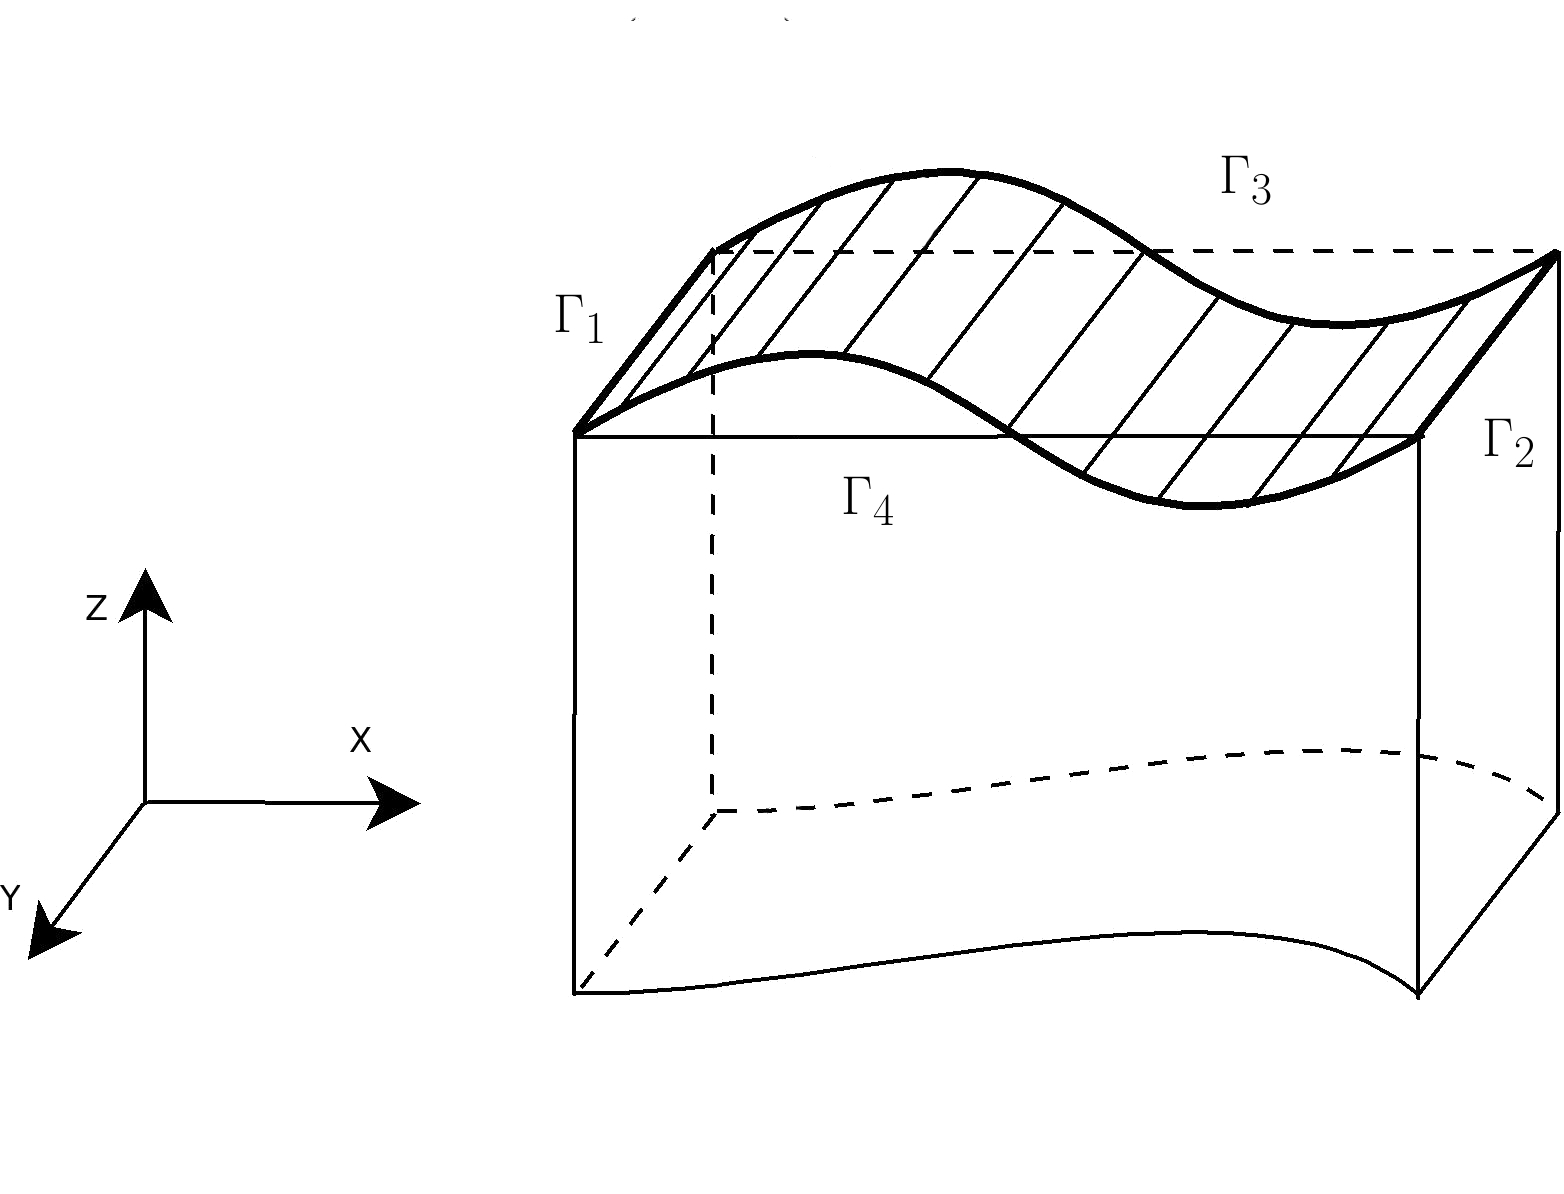
\includegraphics[width=9cm,height=6cm]{boundary_scheme.jpg}
    \caption{Искусственные границы}
    \label{figure:boundary_schema}
\end{figure}

\begin{itemize}

    \item На границе $\Gamma_1=\{x=0,y\in[0,1]\}$
	\begin{eqnarray}
	    \label{eq:ApproxFLinGamma1}
	    F^{n+1}_{lin}=\begin{pmatrix}
		\frac{(H_{1j}-B_{1j}^{n+1})u_{1j}^{n+1}-(H_{0j}-B_{0j}^{n+1})u_{0j}^{n+1}}{2h_x}+\\
		\frac{(H_{0j+1}-B_{0j+1}^{n+1})v_{0j+1}^{n+1}-(H_{0j-1}-B_{0j-1}^{n+1})v_{0j-1}^{n+1}}{2h_y}\\
		\frac{u_{0j}^{n+1}-u_{0j}^{n}}{\tau}+
		g\frac{\eta_{1j}^{n+1}-\eta_{0j}^{n+1}}{2h_x}\\
		\frac{v_{0j}^{n+1}-v_{0j}^{n}}{\tau}+
		g\frac{\eta_{0j+1}^{n+1}-\eta_{0j-1}^{n+1}}{2h_y}
	    \end{pmatrix}
	\end{eqnarray}

	\begin{eqnarray}
	    \label{eq:ApproxFNonlinGamma1}
	    F^{n+1}_{nonlin}=\begin{pmatrix}
		0\\
		v_{0j}\frac{u_{0j+1}^{n+1}-u_{0j-1}^{n}}{2h_y}+
		\frac{(u_{1j}^{n+1})^2-(u_{0j}^{n})^2}{2h_x}\\
		u_{0j}\frac{v_{1j}^{n+1}-v_{0j}^{n}}{2h_x}+
		\frac{(v_{0j+1}^{n+1})^2-(v_{0j-1}^{n})^2}{2h_y}
	    \end{pmatrix}
	\end{eqnarray}

    \item На границе $\Gamma_2=\{x=1,y\in[0,1]\}$
	\begin{eqnarray}
	    \label{eq:ApproxFLinGamma2}
	    F^{n+1}_{lin}=\begin{pmatrix}
		\frac{(H_{n_{x}j}-B_{n_{x}j}^{n+1})u_{n_{x}j}^{n+1}-(H_{n_{x}-1j}-B_{n_{x}-1j}^{n+1})u_{n_{x}-1j}^{n+1}}{2h_x}+\\
		\frac{(H_{n_{x}j+1}-B_{n_{x}j+1}^{n+1})v_{n_{x}j+1}^{n+1}-(H_{n_{x}j-1}-B_{n_{x}j-1}^{n+1})v_{n_{x}j-1}^{n+1}}{2h_y}\\
		\frac{u_{n_{x}j}^{n+1}-u_{n_{x}j}^{n}}{\tau}+
		g\frac{\eta_{n_{x}j}^{n+1}-\eta_{n_{x}-1j}^{n+1}}{2h_x}\\
		\frac{v_{n_{x}j}^{n+1}-v_{n_{x}j}^{n}}{\tau}+
		g\frac{\eta_{n_{x}j+1}^{n+1}-\eta_{n_{x}j-1}^{n+1}}{2h_y}
	    \end{pmatrix}
	\end{eqnarray}

	\begin{eqnarray}
	    \label{eq:ApproxFNonlinGamma2}
	    F^{n+1}_{nonlin}=\begin{pmatrix}
		0\\
		v_{n_{x}j}\frac{u_{n_{x}j+1}^{n+1}-u_{n_{x}j-1}^{n}}{2h_y}+
		\frac{(u_{n_{x}j}^{n+1})^2-(u_{n_{x}-1j}^{n})^2}{2h_x}\\
		u_{n_{x}j}\frac{v_{n_{x}j}^{n+1}-v_{n_{x}-1j}^{n}}{2h_x}+
		\frac{(v_{n_{x}j+1}^{n+1})^2-(v_{n_{x}j-1}^{n})^2}{2h_y}
	    \end{pmatrix}
	\end{eqnarray}

    \item На границе $\Gamma_3=\{x=\in[0,1],y=0\}$
	\begin{eqnarray}
	    \label{eq:ApproxFLinGamma3}
	    F^{n+1}_{lin}=\begin{pmatrix}
		\frac{(H_{i+10}-B_{i+10}^{n+1})u_{i+10}^{n+1}-(H_{i-10}-B_{i-10}^{n+1})u_{i-10}^{n+1}}{2h_x}+\\
		\frac{(H_{i1}-B_{i1}^{n+1})v_{i1}^{n+1}-(H_{i0}-B_{i0}^{n+1})v_{i0}^{n+1}}{2h_y}\\
		\frac{u_{i0}^{n+1}-u_{i0}^{n}}{\tau}+
		g\frac{\eta_{i+10}^{n+1}-\eta_{i-10}^{n+1}}{2h_x}\\
		\frac{v_{i0}^{n+1}-v_{i0}^{n}}{\tau}+
		g\frac{\eta_{i1}^{n+1}-\eta_{i0}^{n+1}}{2h_y}
	    \end{pmatrix}
	\end{eqnarray}

	\begin{eqnarray}
	    \label{eq:ApproxFNonlinGamma3}
	    F^{n+1}_{nonlin}=\begin{pmatrix}
		0\\
		v_{i0}\frac{u_{i1}^{n+1}-u_{i0}^{n}}{2h_y}+
		\frac{(u_{i+10}^{n+1})^2-(u_{i-10}^{n})^2}{2h_x}\\
		u_{i0}\frac{v_{i+10}^{n+1}-v_{i-10}^{n}}{2h_x}+
		\frac{(v_{i1}^{n+1})^2-(v_{i0}^{n})^2}{2h_y}
	    \end{pmatrix}
	\end{eqnarray}

    \item На границе $\Gamma_4=\{x=\in[0,1],y=1\}$
	\begin{eqnarray}
	    \label{eq:ApproxFLinGamma4}
	    F^{n+1}_{lin}=\begin{pmatrix}
		\frac{(H_{i+1n_{y}}-B_{i+1n_{y}}^{n+1})u_{i+1n_{y}}^{n+1}-(H_{i-1n_{y}}-B_{i-1n_{y}}^{n+1})u_{i-1n_{y}}^{n+1}}{2h_x}+\\
		\frac{(H_{in_{y}}-B_{in_{y}}^{n+1})v_{in_{y}}^{n+1}-(H_{in_{y}-1}-B_{in_{y}-1}^{n+1})v_{in_{y}-1}^{n+1}}{2h_y}\\
		\frac{u_{in_{y}}^{n+1}-u_{in_{y}}^{n}}{\tau}+
		g\frac{\eta_{i+1n_{y}}^{n+1}-\eta_{i-1n_{y}}^{n+1}}{2h_x}\\
		\frac{v_{in_{y}}^{n+1}-v_{in_{y}}^{n}}{\tau}+
		g\frac{\eta_{in_{y}}^{n+1}-\eta_{in_{y}-1}^{n+1}}{2h_y}
	    \end{pmatrix}
	\end{eqnarray}

	\begin{eqnarray}
	    \label{eq:ApproxFNonlinGamma4}
	    F^{n+1}_{nonlin}=\begin{pmatrix}
		0\\
		v_{in_{y}}\frac{u_{in_{y}}^{n+1}-u_{in_{y}-1}^{n}}{2h_y}+
		\frac{(u_{i+1n_{y}}^{n+1})^2-(u_{i-1n_{y}}^{n})^2}{2h_x}\\
		u_{in_{y}}\frac{v_{i+1n_{y}}^{n+1}-v_{i-1n_{y}}^{n}}{2h_x}+
		\frac{(v_{in_{y}}^{n+1})^2-(v_{in_{y}-1}^{n})^2}{2h_y}
	    \end{pmatrix}
	\end{eqnarray}

\end{itemize}

Аппроксимация в углах расчетной области выглядит следующим образом:

\begin{itemize}

    \item $x=0\;y=0$
	\begin{eqnarray*}
	    F^{n+1}_{lin}=\begin{pmatrix}
		\frac{(H_{10}-B_{10}^{n+1})u_{10}^{n+1}-(H_{00}-B_{00}^{n+1})u_{00}^{n+1}}{2h_x}+\\
		\frac{(H_{01}-B_{01}^{n+1})v_{01}^{n+1}-(H_{00}-B_{00}^{n+1})v_{00}^{n+1}}{2h_y}\\
		\frac{u_{00}^{n+1}-u_{00}^{n}}{\tau}+
		g\frac{\eta_{10}^{n+1}-\eta_{00}^{n+1}}{2h_x}\\
		\frac{v_{00}^{n+1}-v_{00}^{n}}{\tau}+
		g\frac{\eta_{01}^{n+1}-\eta_{00}^{n+1}}{2h_y}
	    \end{pmatrix}
	\end{eqnarray*}

	\begin{eqnarray*}
	    F^{n+1}_{nonlin}=\begin{pmatrix}
		0\\
		v_{00}\frac{u_{01}^{n+1}-u_{00}^{n}}{2h_y}+
		\frac{(u_{10}^{n+1})^2-(u_{00}^{n})^2}{2h_x}\\
		u_{00}\frac{v_{10}^{n+1}-v_{00}^{n}}{2h_x}+
		\frac{(v_{01}^{n+1})^2-(v_{00}^{n})^2}{2h_y}
	    \end{pmatrix}
	\end{eqnarray*}

    \item $x=1\;y=0$
	\begin{eqnarray*}
	    F^{n+1}_{lin}=\begin{pmatrix}
		\frac{(H_{n_{x}0}-B_{n_{x}0}^{n+1})u_{n_{x}0}^{n+1}-(H_{n_{x}-10}-B_{n_{x}-10}^{n+1})u_{n_{x}-10}^{n+1}}{2h_x}+\\
		\frac{(H_{n_{x}1}-B_{n_{x}1}^{n+1})v_{n_{x}1}^{n+1}-(H_{n_{x}0}-B_{n_{x}0}^{n+1})v_{n_{x}0}^{n+1}}{2h_y}\\
		\frac{u_{n_{x}0}^{n+1}-u_{n_{x}0}^{n}}{\tau}+
		g\frac{\eta_{n_{x}0}^{n+1}-\eta_{n_{x}-10}^{n+1}}{2h_x}\\
		\frac{v_{n_{x}0}^{n+1}-v_{n_{x}0}^{n}}{\tau}+
		g\frac{\eta_{n_{x}1}^{n+1}-\eta_{n_{x}0}^{n+1}}{2h_y}
	    \end{pmatrix}
	\end{eqnarray*}

	\begin{eqnarray*}
	    F^{n+1}_{nonlin}=\begin{pmatrix}
		0\\
		v_{n_{x}0}\frac{u_{n_{x}1}^{n+1}-u_{n_{x}0}^{n}}{2h_y}+
		\frac{(u_{n_{x}0}^{n+1})^2-(u_{n_{x}-10}^{n})^2}{2h_x}\\
		u_{n_{x}0}\frac{v_{n_{x}0}^{n+1}-v_{n_{x}-10}^{n}}{2h_x}+
		\frac{(v_{n_{x}1}^{n+1})^2-(v_{n_{x}0}^{n})^2}{2h_y}
	    \end{pmatrix}
	\end{eqnarray*}

    \item $x=0\;y=1$
	\begin{eqnarray*}
	    F^{n+1}_{lin}=\begin{pmatrix}
		\frac{(H_{1n_{y}}-B_{1n_{y}}^{n+1})u_{1n_{y}}^{n+1}-(H_{0n_{y}}-B_{0n_{y}}^{n+1})u_{0n_{y}}^{n+1}}{2h_x}+\\
		\frac{(H_{0n_{y}}-B_{0n_{y}}^{n+1})v_{0n_{y}}^{n+1}-(H_{0n_{y}-1}-B_{0n_{y}-1}^{n+1})v_{0n_{y}-1}^{n+1}}{2h_y}\\
		\frac{u_{0n_{y}}^{n+1}-u_{0n_{y}}^{n}}{\tau}+
		g\frac{\eta_{1n_{y}}^{n+1}-\eta_{0n_{y}}^{n+1}}{2h_x}\\
		\frac{v_{0n_{y}}^{n+1}-v_{0n_{y}}^{n}}{\tau}+
		g\frac{\eta_{0n_{y}}^{n+1}-\eta_{0n_{y}-1}^{n+1}}{2h_y}
	    \end{pmatrix}
	\end{eqnarray*}

	\begin{eqnarray*}
	    F^{n+1}_{nonlin}=\begin{pmatrix}
		0\\
		v_{0n_{y}}\frac{u_{0n_{y}}^{n+1}-u_{0n_{y}-1}^{n}}{2h_y}+
		\frac{(u_{1n_{y}}^{n+1})^2-(u_{0n_{y}}^{n})^2}{2h_x}\\
		u_{0n_{y}}\frac{v_{1n_{y}}^{n+1}-v_{0n_{y}}^{n}}{2h_x}+
		\frac{(v_{0n_{y}}^{n+1})^2-(v_{0n_{y}-1}^{n})^2}{2h_y}
	    \end{pmatrix}
	\end{eqnarray*}

    \item $x=1\;y=1$
	\begin{eqnarray*}
	    F^{n+1}_{lin}=\begin{pmatrix}
		\frac{(H_{n_{x}n_{y}}-B_{n_{x}n_{y}}^{n+1})u_{n_{x}n_{y}}^{n+1}-(H_{n_{x}-1n_{y}}-B_{n_{x}-1n_{y}}^{n+1})u_{n_{x}-1n_{y}}^{n+1}}{2h_x}+\\
		\frac{(H_{n_{x}n_{y}}-B_{n_{x}n_{y}}^{n+1})v_{n_{x}n_{y}}^{n+1}-(H_{n_{x}n_{y}-1}-B_{n_{x}n_{y}-1}^{n+1})v_{n_{x}n_{y}-1}^{n+1}}{2h_y}\\
		\frac{u_{n_{x}n_{y}}^{n+1}-u_{n_{x}n_{y}}^{n}}{\tau}+
		g\frac{\eta_{n_{x}n_{y}}^{n+1}-\eta_{n_{x}-1n_{y}}^{n+1}}{2h_x}\\
		\frac{v_{n_{x}n_{y}}^{n+1}-v_{n_{x}n_{y}}^{n}}{\tau}+
		g\frac{\eta_{n_{x}n_{y}}^{n+1}-\eta_{n_{x}n_{y}-1}^{n+1}}{2h_y}
	    \end{pmatrix}
	\end{eqnarray*}

	\begin{eqnarray*}
	    F^{n+1}_{nonlin}=\begin{pmatrix}
		0\\
		v_{ij}\frac{u_{ij+1}^{n+1}-u_{ij-1}^{n}}{2h_y}+
		\frac{(u_{i+1j}^{n+1})^2-(u_{i-1j}^{n})^2}{2h_x}\\
		u_{ij}\frac{v_{i+1j}^{n+1}-v_{i-1j}^{n}}{2h_x}+
		\frac{(v_{ij+1}^{n+1})^2-(v_{ij-1}^{n})^2}{2h_y}
	    \end{pmatrix}
	\end{eqnarray*}

\end{itemize}

\newpage
\addtocounter{section}{1}
\setcounter{subsection}{0}
\setcounter{equation}{0}
\section*{Алгоритм решения}
\addtocontents{toc}{\contentsline{section}{\protect\numberline{\S\;\thesection.}\vspace{10pt}Алгоритм решения}{\thepage}}

В итоге, схема (\ref{eq:ApproxMainEq})-(\ref{eq:ApproxFNonlin}) с замыканием на $\Gamma$ представляет собой систему нелинейных алгебраических уравнений (СНАУ)

\begin{gather}
    AU=f\notag\\
    A=A_{lin}+A_{nonlin}
    \label{eq:MainSolveEq}
\end{gather}
относительно переменных $U^n=(\eta^{n+1}_{00},\ldots,\eta^{n+1}_{n_xn_y},u^{n+1}_{00},\ldots,u^{n+1}_{n_xn_y},v^{n+1}_{00},\ldots,v^{n+1}_{n_xn_y0})$, где вектор $f$ известен и зависит от $\eta^{n+1}_{ij},u^{n+1}_{ij},v^{n+1}_{ij},H_{ij},B^{n+1}_{ij},B^{n}_{ij}$, а $A_{lin}$ - оператор аппроксимации линейной части (\ref{eq:MainVectorForm})-(\ref{eq:BoundaryCondition}), $A_{nonlin}$ - оператор аппроксимации нелинейной части (\ref{eq:MainVectorForm})-(\ref{eq:BoundaryCondition}).

Для решения задачи (\ref{eq:MainVectorForm})-(\ref{eq:BoundaryCondition}) использовался следующий алгоритм:
\begin{itemize}
    \item По известному вектору $\{u_{ij}^n,v_{ij}^n,\eta_{ij}^n\}$ на каждом временном слое каким-либо итерационным методом находим приближенное решение системы (\ref{eq:MainSolveEq}).
    \item Оно принимается за решение схемы (\ref{eq:ApproxMainEq})-(\ref{eq:ApproxFNonlin}) на n+1 слое.
\end{itemize}

Матрица полученной системы уравнений не обладает свойствами, необходимыми для решения системы известными методами, поэтому для ее решения мы воспользовались методом неполной аппроксимации минимальных невязок, шаг которого выглядит следующим образом:

\begin{equation}
    \label{FirstMethodStep}
    u^{k+\frac{1}{2}}=u^k-\tau_{k+1}r^k\\
\end{equation}
\begin{equation}
    \label{SecondMethodStep}
    u^{k+1}=u^{k+\frac{1}{2}}-\alpha_{k+1}z^k
\end{equation}

где $\tau$ - итерационный параметр, выбираемый из условия минимума $\|r^{k+\frac{1}{2}}\|$,$z^k$ - заданный вектор,$\alpha$ - матрица итерационных параметров, элементы которой выбираются из минимума последовательности норм невязок.

\newpage
\addtocounter{section}{1}
\setcounter{subsection}{0}
\setcounter{equation}{0}
\section*{Описание двухслойной схемы неполной аппроксимации}
\addtocontents{toc}{\contentsline{section}{\protect\numberline{\S\;\thesection.}\vspace{10pt}Описание двухслойной схемы неполной аппроксимации}{\thepage}}

Пусть в конечномерном вещественном гильбертовом пространстве $H_m$ задана система уравнений
\begin{equation}
    \label{eq:MainMethodSystem}
    Au=f
\end{equation}
с невырожденной незнакоопределенной матрицей $A=(a_{ij})$ порядка $m$. Здесь $u,f$ - неизвестный и известный $m$-мерные векторы из $H_m$.

В дальнейшем будем считать, что $det A$ или одно из собственных чисел могут быть близкими к машинному нулю. Если матрица незнакоопределена, то, умножая систему (\ref{eq:MainMethodSystem}) на $A^*$ (1-ая трансформация Гаусса), получим новую систему с положительно определенной матрицей $\overline{A}=A^{*}A$ и правой частью $A^{*}f$. Для решения этой системы можно использовать достаточно широкий арсенал итерационных схем, но в нашем случае такой путь решения системы (\ref{eq:MainMethodSystem}) не приемлем, т.к. $det A$ или одно из собственных чисел могут быть близкими к машинному нулю.

Для решения системы (\ref{eq:MainMethodSystem}) рассмотрим итерационную схему неполной аппроксимации (более подробное описание метода см. \cite{zakharov})
\begin{equation}
    \label{eq:FirstTheoryMethodStep}
    u^{n+\frac{1}{2}}=u^n-\tau_{n+1}B(Au^n-f)\\
\end{equation}
\begin{equation}
    \label{eq:SecondTheoryMethodStep}
    u^{n+1}=u^{n+\frac{1}{2}}-\alpha_{n+1}z^n,\;n=0,1,2,\ldots
\end{equation}
где $B$ - неособенная квадратная матрица, $z^n\in H_m$ - произвольный вектор, $\tau_{n+1},\alpha_{n+1}$ -итерационные параметры, $u^0$ - произвольный начальный вектор. Заметим, что $\alpha_{n+1}$ может быть как константой, так и матрицей.

\addtocounter{subsection}{1}
\subsection*{Случай, когда $\alpha_{n+1}=const$}
\addtocontents{toc}{\contentsline{subsection}{\protect\numberline{\thesubsection.}\vspace{10pt}Случай, когда $\alpha_{n+1}=const$}{\thepage}}

Пусть в схеме (\ref{eq:FirstTheoryMethodStep})-(\ref{eq:SecondTheoryMethodStep}) $\alpha_{n+1}=const$,а $D$ - самосопряженный положительно определенный оператор, дейтсвующий в $H_m$. Тогда относительно $v^n=D^{\frac{1}{2}}(u^n-u)$ система имеет вид

\begin{equation}
    \label{eq:FirstTheoryMethodStepResidual}
    v^{n+\frac{1}{2}}=S_{n+1}v^n\\
\end{equation}
\begin{equation}
    \label{eq:SecondTheoryMethodStepResidual}
    v^{n+1}=v^{n+\frac{1}{2}}-\alpha_{n+1}D^{\frac{1}{2}}z^n,\;n=0,1,2,\ldots
\end{equation}
где $S_{n+1}=E-\tau_{n+1}C,\; C=D^{\frac{1}{2}}z^n,\; v^{n+\frac{1}{2}}=D^{\frac{1}{2}}(u^{n+\frac{1}{2}}-u)$.

Тогда 
\begin{equation}
    \label{eq:TheoryMethodResidual1}
    \|v^{n+1}\|^2=\|v^{n+\frac{1}{2}}\|^2-2\alpha_{n+1}(v^{n+\frac{1}{2}},D^{\frac{1}{2}}z^n)+\alpha^2_{n+1}\|D^{\frac{1}{2}}z^n\|^2
\end{equation}

Если вектор $z^n$ такой, что $D^{\frac{1}{2}}z^n\neq 0$, то, выбирая $\alpha_{n+1}$ из условия минимума $\|v^{n+1}\|^2$, получаем
\begin{equation}
    \label{eq:TheoryMethodResidual2}
    \|v^{n+1}\|^2=\|v^{n+\frac{1}{2}}\|^2-\frac{(v^{n+\frac{1}{2}},D^{\frac{1}{2}}z^n)^2}{\|D^{\frac{1}{2}}z^n\|^2}
\end{equation}
при
\begin{equation}
    \label{eq:TheoryMethodAlpha}
    \alpha_{n+1}=\frac{(v^{n+\frac{1}{2}},D^{\frac{1}{2}}z^n)^2}{\|D^{\frac{1}{2}}z^n\|^2}
\end{equation}

Параметр $\tau_{n+1}$, например, можно выбирать из условия минимума $\|v^{n+\frac{1}{2}}\|^2$
\begin{equation}
    \label{eq:TheoryMethodResidual3}
    \|v^{n+\frac{1}{2}}\|^2=\|v^{n}\|^2-2\tau_{n+1}(v^{n},Cv^n)+\tau^2_{n+1}\|Cv^n\|^2
\end{equation}
тогда
\begin{equation}
    \label{eq:TheoryMethodTau}
    \tau_{n+1}=\frac{(Cv^{n},v^n)}{\|Cv^n\|^2}
\end{equation}
и формулу (\ref{eq:TheoryMethodResidual2}) можно пререписать в виде

\begin{equation}
    \label{eq:TheoryMethodResidualSimple}
    \|v^{n+1}\|^2=\Theta^{(1)}_{n+1}\|v^n\|^2
\end{equation}
где
\begin{equation}
    \label{eq:TheoryMethodResidualLessOne}
    \Theta^{(1)}_{n+1}=\rho^2_{n+1}-R_{n+1}\leq1
\end{equation}

\begin{equation}
    \label{eq:TheoryMethodResidualR}
    R_{n+1}=\frac{v^{n+\frac{1}{2}},D^{\frac{1}{2}}z^n)^2}{\|D^{\frac{1}{2}}z^n\|^2\|v^n\|^2}
\end{equation}

\begin{equation}
    \label{eq:TheoryMethodResidualRho}
    \rho^2_{n+1}=1-\frac{Cv^n,v^n)^2}{\|Cv^n\|^2\|v^n\|^2}
\end{equation}

Справедлива
\begin{Theorem}
    Если для всех $n$ вектор $z^n$ такой, что $(D^{\frac{1}{2}}v^{n+\frac{1}{2}},z^n)\neq 0$, то итерационная схема (\ref{eq:TheoryMethodResidual1}),\\(\ref{eq:TheoryMethodAlpha}),(\ref{eq:TheoryMethodTau}) сходится, т.е $\|v^{n+1}\|to 0$ при $n\to \infty$ для любого $v_0$
\end{Theorem}

В \cite{zakharov} показано, что строить векторы $z^n$ такие, чтобы для величины $\Theta^{(1)}_{n}$ выполнялась оценка $\Theta^{(1)}_{n}\leq\;\Theta_{*}<1$, достаточно просто.

\begin{Theorem}
    Итерационная схема (\ref{eq:TheoryMethodResidual1}),(\ref{eq:TheoryMethodAlpha}),(\ref{eq:TheoryMethodTau}) является сходящейся, если задать вектор $z^n$ в виде
    \begin{equation*}
	z^n=x^n+\frac{\sigma}{(D^{\frac{1}{2}}v^{\frac{1}{2}},v^{\frac{1}{2}})}v^{n+\frac{1}{2}}
    \end{equation*}
    со следующей оценкой:
    \begin{equation}
	\|v^{n+1}\|^2\leq(1-\xi)\rho^2_{n+1}\|v^n\|^2
    \end{equation}
    где $\xi = \frac{\gamma_1}{\gamma_2}$, a $\rho^2_{n+1}$ определяется равенством (\ref{eq:TheoryMethodResidualRho})
\end{Theorem}

\addtocounter{subsection}{1}
\subsection*{Случай, когда $\alpha_{n+1}$ является матрицей}
\addtocontents{toc}{\contentsline{subsection}{\protect\numberline{\thesubsection.}\vspace{10pt}Случай, когда $\alpha_{n+1}$ является матрицей}{\thepage}}

Для схемы (\ref{eq:FirstTheoryMethodStep})-(\ref{eq:SecondTheoryMethodStep}) введем параметр $\alpha_{n+1}$ в виде диагональной матрицы размерности $m$.

Пусть $z^n$ - вектор, все элементы которого равны единице, тогда произведение $\alpha_{n+1}z^n$ можно представить в виде
\begin{equation}
    \label{eq:AlphaZSumm}
    \alpha_{n+1}z^n=\sum^m_{i=1}\alpha^i_{n+1}z^n_i
\end{equation}
где $\alpha^i_{n+1}$ - элемент главной диагонали матрицы $a_{}n+1$, стоящий в $i$-й строке, $z^n_i$ - вектор с ненулевой $i$-й компонентой. Следовательно,

\begin{equation}
    \label{eq:VAlphaDZSumm}
    v^{n+1}=v^{n+\frac{1}{2}}-\sum^m_{i=1}\alpha^i_{n+1}D^{\frac{1}{2}}z^n_i
\end{equation}

Будем находить элементы матрицы $\{\alpha^i_{n+1}\}$ из условия минимума $\|v^{n+1}\|$
\begin{equation}
    \label{eq:MinNormaV}
    \|v^{n+1}\|^2=\|v^{n+\frac{1}{2}}\|^2-\sum^m_{i=1}\alpha^i_{n+1}(v^{n+\frac{1}{2}},D^{\frac{1}{2}}z^n_i)+\sum^m_{i=1}\sum^m_{j=1}\alpha^i_{n+1}\alpha^j_{n+1}(D^{\frac{1}{2}}z^n_i,D^{\frac{1}{2}}z^n_j)
\end{equation}

Для функций многих переменных справедлива
\begin{Theorem}
    Если $f(x)\in C^2(R^m)$, где $x\in R^m$, и выполнено условие
    \begin{equation}
	\frac{\partial f}{\partial x_i}(x_0)=0
    \end{equation}
    а также $d^2_{xx}f(x_0)$ - матрица частных производных второго порядка строго полодительно определена, то точка $x_0$ является точкой глобального минимума
\end{Theorem}

В \cite{zakharov} показано, что все условия теоремы выполняются, т.к. по условию матрица $D$ положительно определенная и неособенная, а векторы $\{z^n_m\}$ по построению линейно независимы.

\addtocounter{subsection}{1}
\subsection*{Метод минимальных невязок}
\addtocontents{toc}{\contentsline{subsection}{\protect\numberline{\thesubsection.}\vspace{10pt}Метод минимальных невязок}{\thepage}}

Пусть $D=A^*A$, тогда (\ref{eq:SecondTheoryMethodStepResidual}) перепишется в виде
\begin{equation}
    \label{eq:SecondTheoryMethodStepResidual2}
    v^{n+1}=v^{n+\frac{1}{2}}-\alpha_{n+1}(A^*A)^{\frac{1}{2}}z^n,\;n=0,1,2,\ldots
\end{equation}
и минимизируя $\|r^{n+1}\|$, получим

\begin{equation}
    \label{eq:TheoryMethodAlpha2}
    \alpha_{n+1}=\frac{(r^{n+\frac{1}{2}},Az^n)}{\|Az^n\|^2}
\end{equation}

Если же $\alpha_{n+1}$ - диагональная матрица, то ее элементы будем находить как решение системы
\begin{equation}
    \label{eq:TheoryMethodAlpha3}
    \begin{pmatrix}
	(Az^n_1,Az^n_1) & (Az^n_1,Az^n_2) & \cdots & (Az^n_1,Az^n_m)\\
	(Az^n_2,Az^n_1) & (Az^n_2,Az^n_2) & \cdots & (Az^n_2,Az^n_m)\\
	\vdots & \vdots & & \vdots\\
	(Az^n_m,Az^n_1) & (Az^n_m,Az^n_2) & \cdots & (Az^n_m,Az^n_m)\\
    \end{pmatrix}
    \times
    \begin{pmatrix}
	\alpha^1_{n+1}\\
	\alpha^2_{n+1}\\
	\vdots\\
	\alpha^m_{n+1}\\
    \end{pmatrix}
    =
    \begin{pmatrix}
	(Az^n_1,r^n)\\
	(Az^n_2,r^n)\\
	\vdots\\
	(Az^n_m,r^n)\\
    \end{pmatrix}\notag
\end{equation}
